\documentclass[10pt]{jarticle}
\usepackage{float}
\usepackage{adrobo_abst}
\usepackage[dvipdfmx]{graphicx}
\usepackage{amssymb,amsmath}
\usepackage{bm}
\usepackage[superscript]{cite}
\usepackage{enumerate}
\usepackage{url}
\usepackage{comment}
%\usepackage[absolute]{textpos}

\setlength\intextsep{5pt}
\setlength\textfloatsep{5pt}

\renewcommand\citeform[1]{(#1)}

\graphicspath{{../fig/}}

\begin{document}
    
    \makeatletter
    \doctype{2025年度卒業論文概要}
    \title{磁気吸着を用いた壁面走行型塗膜剥離ロボットの開発}{}
    \etitle{Development of a Magnetically Adhered Wall-Climbing Robot for Paint Peeling}{}
    
    \author{22C1089\hspace{.5zw}床枝純}
    \eauthor{Jun TOKOEDA}
    
    \makeatother
    
    \abstract{This paper describes the development of a magnetically adhered wall-climbing robot equipped with a scraper mechanism for paint removal on steel bridge surfaces.Conventional paint removal work requires significant manual labor under harsh conditions.To reduce the physical burden on workers, a robot capable of adhering to steel surfaces and moving stably on vertical walls was developed.The proposed robot uses magnetic adhesion for wall-climbing locomotion and a scraper mechanism whose blade angle can be adjusted by a linear actuator.Experiments were conducted on an actual steel bridge surface after paint heating.As a result, stable wall-climbing locomotion was achieved.Although continuous paint removal by self-propelled scraping was difficult due to insufficient driving torque and adhesion force, paint removal was successfully performed after an initial insertion of the scraper.These results clarify the requirements for adhesion force and blade angle control in scraper-based paint removal robots.
    }

    \keywords{Wall-climbing robot, Magnetic adhesion, Paint removal, Scraper mechanism}

    \maketitle
    
    \supervisor{指導教員：米田完 教授}
    
    \section{緒\hspace{2zw}言}%===========================
    
    
    鋼橋の塗替え工事における塗膜剥離作業は，作業者に大きな身体的負担を強いる作業であり，
    作業環境の改善および省力化が求められている．
    近年，高周波誘導加熱を用いた塗膜除去技術が実用化されているが，
    加熱後の塗膜剥離作業は依然として人手に依存している．
    
    これまでに，磁気吸着を用いた壁面走行ロボットによる加熱作業の研究が行われてきたが，
    加熱後の塗膜を自動的に剥離する機構については十分な検討がなされていない．
    そこで本研究では，磁気吸着により鋼橋壁面を走行可能なロボットに，
    スクレーパ式塗膜剥離機構を搭載し，その有効性について検討する．

    \section{研究目標}%===========================
    以下に表記する, 作業空間で想定される環境を走破可能である事を目標とする.

	・土地盤（礫, 砂, シルト, 粘土）（含水率は不定）
	
    ・現場ヤード（アスファルト, コンクリート, 鉄板）

    ・土地盤と現場ヤードの境目などで生じる高低差

    \section{機体構想}
    旋回時に地面を掘る原因として, 各クローラ回転時のベクトルと機体が進むベクトルの角度に大きな差が生じる事で, 横方向に滑る力が働く事が考えられる.
    そして機体が進むベクトルと同方向に推力を加える駆動部や段差踏破機構がない為, スタックしてしまう.
    
    各駆動部の向きを円形に変形させ, 推力のベクトルを円の接線方向に向ける事でスタックを防ぐ事が可能だと考えられる.

    変形する為には駆動部の側面は極力短くして地面を掘る面積を抑える必要がある.
    よって本機体ではクローラではなく車輪を採用し, 駆動部はユニットに分割する方式を採用した.
    変形には機体の両側に多重歯車を使用している.
    機体概要を図 \ref{friction3}に示す.


    \begin{figure}[H]
        \centering
        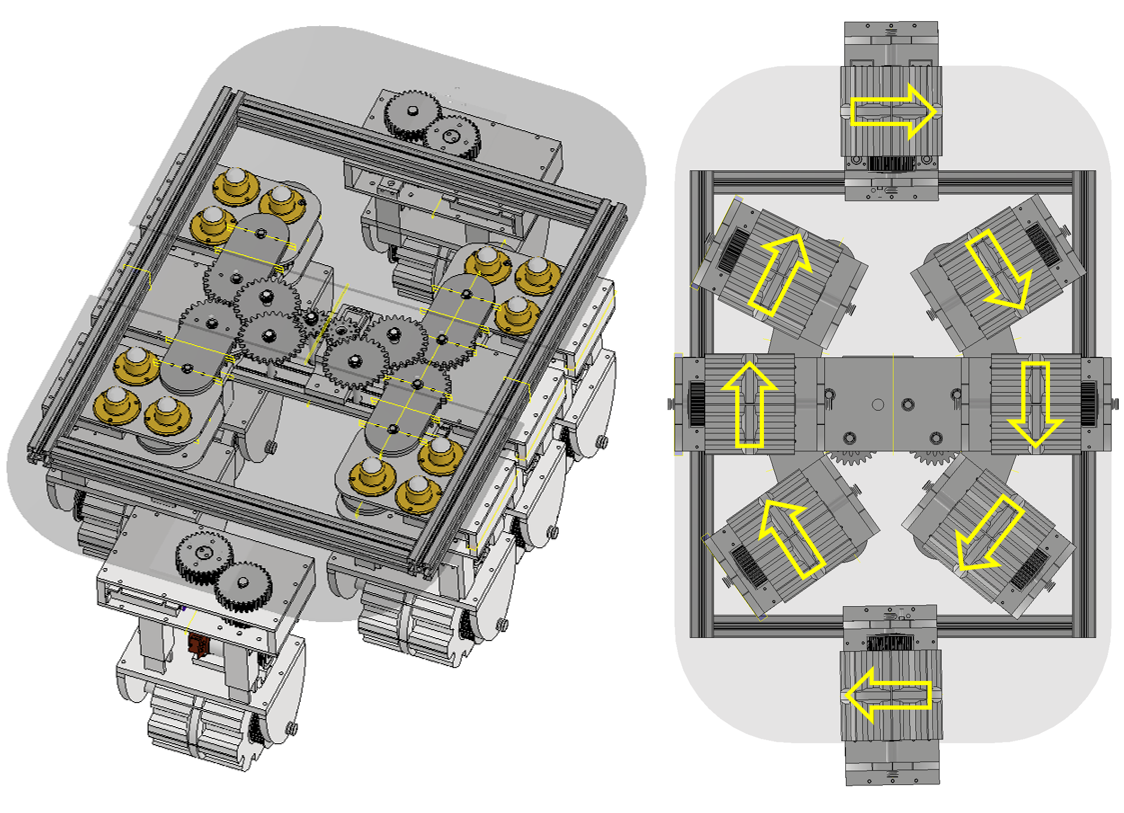
\includegraphics[width=0.45\textwidth]{image_1_2.png}
        \vspace{-3mm}
        \caption{machine blueprint}
        \label{friction3}
    \end{figure}

    \newpage
    
    \section{機体製作}
    先述の構想を元に製作した機体を図 \ref{prot1}に示す.

    機体のアスペクト比は現在使用されているクローラ型ロボットと同様, 約1.6 : 1 で製作を行った.

    本機体には段差による影響を減らし, 走行時に全ての車輪を接地させる為, 各ユニットごとにサスペンションを搭載した.

    電源を除く機体諸元を表 \ref{specification}に示す.
    

    \begin{figure}[h]
        \centering
        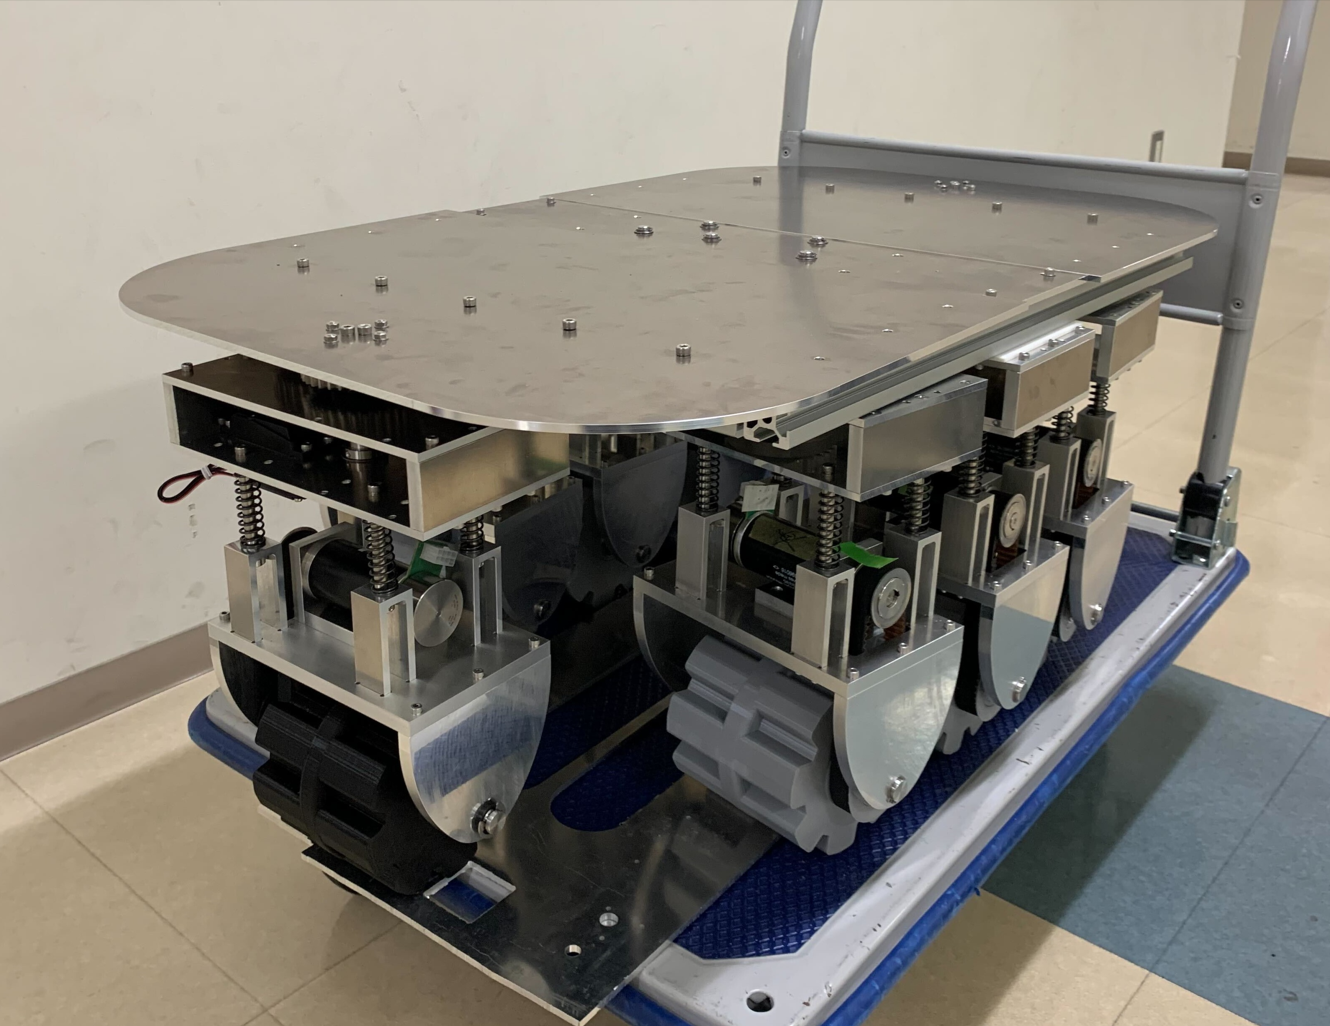
\includegraphics[width=0.45\textwidth]{robot_1_1.png}
        \vspace{-3mm}
        \caption{produced machine}
        \label{prot1}
    \end{figure}

    \begin{table}[h]
        \centering
        \caption{Specification of machine}
        \vspace{1mm}
        \begin{tabular}{cc} \hline
          Length & 870[mm] \\
          Width & 560[mm] \\
          Height & 360[mm] \\ 
          Weight & 57.8[kg] \\ \hline
        \end{tabular}
        \label{specification}
      \end{table}
   

    走行環境は鉄板などの硬質な素材から含水率の高い流体状の地面まで様々である為, 様々な環境に合わせた特殊な形状の車輪を設計した.
    図 \ref{prot2}に示す.

    泥濘地の走行では, 接地面積の少なさを改善するために溝を作り表面積を増やした. さらに走行時に溝で泥を掻く事で, より推力を出す事ができると考える.
    
    硬質な素材上では点接地の方が摩擦を軽減できて走行効率が上がる為, 車輪中央のみ溝を無くしている.


    \begin{figure}[h]
        \centering
        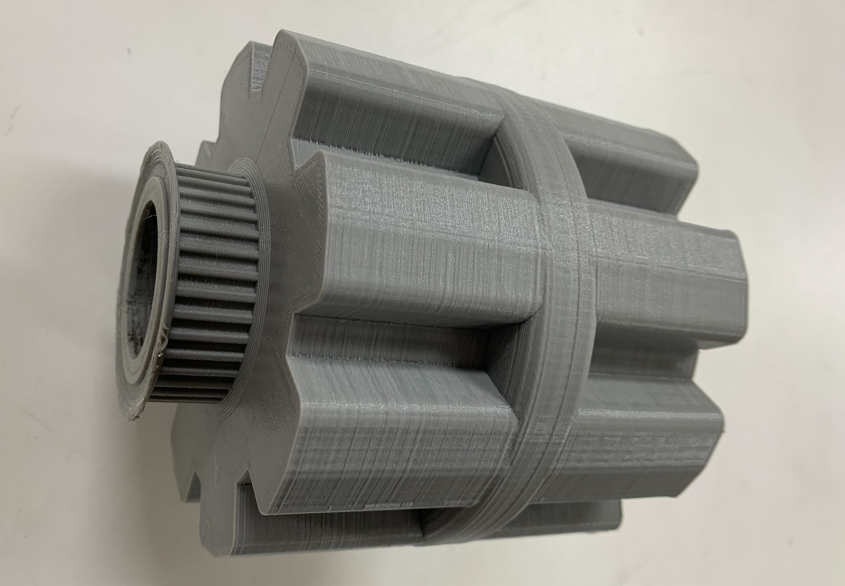
\includegraphics[width=0.45\textwidth]{robot_1_3.png}
        \vspace{-3mm}
        \caption{special shaped wheels}
        \label{prot2}
    \end{figure}



    \section{機体の性能実験}
    今回は現場ヤードでの走行性能を検証するために, 想定環境での走行実験と段差踏破の実験を行った.

    \subsection{走行実験}
    走行実験において走行スピードはモータの性能とプログラムに依存する為, モータの性能から出される理論値との比較を行う. なお今回の実験には機体重量によるモータへの負荷や実験環境による外力は考慮しないものとする.
    
    結果を表 \ref{friction}に示す.
    \vspace{-2mm}

    \begin{table}[h]
        \centering
        \caption{Driving experiment}
        \begin{tabular}{ccc}
        environment           & distance traveled      \\ \hline
        theoretical value     & 26.53 [mm/s]            \\
        iron plate            & 24.39 [mm/s]            \\
        concrete              & 25.64 [mm/s]            \\
        asphalt               & 26.32 [mm/s]
        \end{tabular}
        \label{friction}
    \end{table}
    
    実験の結果, 理論値よりも低い性能であるが, 外力の影響も含めると理論値に近い性能を出す事ができた.

    \subsection{段差踏破実験}
    車輪数の多い機体には段差踏破時のタイムロスが考えられるため, 踏破可能な高さと走行時間の実験を行った.
    
    結果を表 \ref{friction2}に示す.
    \vspace{-2mm}

    \begin{table}[h]
        \centering
        \caption{Step-crossing experiment}
        \begin{tabular}{ccc}
        step height    & crossing time     & turning time  \\ \hline
        0 [mm]          & 32 [s]       & 26 [s]          \\
        6 [mm]          & 32 [s]       & 24 [s]          \\
        12 [mm]         & 33 [s]       & 28 [s]          \\
        18 [mm]         & 32 [s]       & 27 [s]          \\
        24 [mm]         & 34 [s]       & 29 [s]
        \end{tabular}
        \label{friction2}
    \end{table}

    実験の結果, 段差の高さによる走行スピードへの影響はほとんどなかった.
    サスペンションにより, タイムロスを抑える事ができたと考えられる.

    \section{結\hspace{2zw}言}
    本研究では泥濘地でのスタックを防止するため, 各車輪の方向を進行方向にそろえる機構をもつ8輪運搬ロボットの提案と製作を行った.
    また現場ヤードを想定した検証を行った.
    
    検証の結果, 平地走行や段差踏破では十分な性能を持つことが検証できた.

    今後は土地盤で含水率を変えつつ走行実験を行い, 泥濘地でのスタック防止機構の有用性の評価を行う.


    \vspace{5truemm}
    {\footnotesize
        \begin{thebibliography}{99}

            \bibitem{magnetic-clawlar2} 
	        工法の概要|オリエンタル白石株式会社
	        
            \url{https://www.orsc.co.jp/tec/newm_v2/ncon02.html}
	        
            （参照日 2024年1月19日）
            
        \end{thebibliography}
    }
    \normalsize
    
\end{document}